% Capitolul 1: Introducere în Analiza Seriilor de Timp
% Prezentare academică de calitate Harvard
% Program de licență, Academia de Studii Economice din București

\documentclass[9pt, aspectratio=169, t]{beamer}

% Asigură încadrarea conținutului pe diapozitive
\setbeamersize{text margin left=8mm, text margin right=8mm}

%=============================================================================
% CONFIGURARE TEMĂ ȘI STIL
%=============================================================================
\usetheme{default}
% Using default theme for clean header/footer control

% Paleta de culori (matching Redispatch PDF)
\definecolor{MainBlue}{RGB}{26, 58, 110}
\definecolor{AccentBlue}{RGB}{26, 58, 110}
\definecolor{IDAred}{RGB}{205, 0, 0}
\definecolor{DarkGray}{RGB}{51, 51, 51}
\definecolor{MediumGray}{RGB}{128, 128, 128}
\definecolor{LightGray}{RGB}{248, 248, 248}
\definecolor{VeryLightGray}{RGB}{235, 235, 235}
\definecolor{KeynoteGray}{RGB}{218, 218, 218}
\definecolor{SectionGray}{RGB}{120, 120, 120}
\definecolor{FooterGray}{RGB}{100, 100, 100}
\definecolor{Crimson}{RGB}{220, 53, 69}
\definecolor{Forest}{RGB}{46, 125, 50}
\definecolor{Amber}{RGB}{181, 133, 63}
\definecolor{Orange}{RGB}{230, 126, 34}
\definecolor{Purple}{RGB}{142, 68, 173}

% Fundal gradient (gradient Keynote exact 315°: alb la RGB 218,218,218)
\setbeamertemplate{background}{%
    \begin{tikzpicture}[remember picture, overlay]
        \shade[shading=axis, shading angle=315,
        top color=white, bottom color=KeynoteGray]
        (current page.south west) rectangle (current page.north east);
    \end{tikzpicture}%
}
% Culoare solidă de rezervă pentru compatibilitate
\setbeamercolor{background canvas}{bg=}

\setbeamercolor{palette primary}{bg=MainBlue, fg=white}
\setbeamercolor{palette secondary}{bg=MainBlue!85, fg=white}
\setbeamercolor{palette tertiary}{bg=MainBlue!70, fg=white}
\setbeamercolor{structure}{fg=MainBlue}
\setbeamercolor{title}{fg=IDAred}
\setbeamercolor{frametitle}{fg=IDAred, bg=}
\setbeamercolor{block title}{bg=MainBlue, fg=white}
\setbeamercolor{block body}{bg=VeryLightGray, fg=DarkGray}
\setbeamercolor{block title alerted}{bg=Crimson, fg=white}
\setbeamercolor{block body alerted}{bg=Crimson!8, fg=DarkGray}
\setbeamercolor{block title example}{bg=Forest, fg=white}
\setbeamercolor{block body example}{bg=Forest!8, fg=DarkGray}
\setbeamercolor{item}{fg=MainBlue}

% Culori subsol (suprascrie albastrul temei Madrid)
\setbeamercolor{author in head/foot}{fg=FooterGray, bg=}
\setbeamercolor{title in head/foot}{fg=FooterGray, bg=}
\setbeamercolor{date in head/foot}{fg=FooterGray, bg=}
\setbeamercolor{section in head/foot}{fg=FooterGray, bg=}
\setbeamercolor{subsection in head/foot}{fg=FooterGray, bg=}

% Stiluri pentru bullet-uri (se aplică peste tot, inclusiv în blocuri)
\setbeamertemplate{itemize item}{\color{MainBlue}$\boxdot$}
\setbeamertemplate{itemize subitem}{\color{MainBlue}$\blacktriangleright$}
\setbeamertemplate{itemize subsubitem}{\color{MainBlue}\tiny$\bullet$}
\setbeamertemplate{itemize/enumerate body begin}{\normalsize}
\setbeamertemplate{itemize/enumerate subbody begin}{\normalsize}

% Item spacing - compact style
\setlength{\leftmargini}{10pt}       % Level 1: minimal indent
\setlength{\leftmarginii}{10pt}      % Level 2: minimal additional indent
% Compact list spacing (zero extra space before/after lists in blocks)
\makeatletter
\def\@listi{\leftmargin\leftmargini \topsep 0pt \parsep 0pt \itemsep 0pt}
\def\@listii{\leftmargin\leftmarginii \topsep 0pt \parsep 0pt \itemsep 0pt}
\makeatother

\setbeamertemplate{navigation symbols}{}

%=============================================================================
% ANTET PERSONALIZAT
%=============================================================================
\setbeamertemplate{headline}{%
    \vskip10pt%
    \hbox to \paperwidth{%
        \hskip0.5cm%
        {\small\color{FooterGray}\renewcommand{\hyperlink}[2]{##2}\insertsectionhead}%
        \hfill%
        \textcolor{FooterGray}{\small\insertframenumber}%
        \hskip0.5cm%
    }%
    \vskip4pt%
    {\color{FooterGray}\hrule height 0.4pt}%
}

%=============================================================================
% SUBSOL PERSONALIZAT
%=============================================================================
\usepackage{fontawesome5}

\setbeamertemplate{footline}{%
    {\color{FooterGray}\hrule height 0.4pt}%
    \vskip4pt%
    \hbox to \paperwidth{%
        \hskip0.5cm%
        \textcolor{FooterGray}{\small Analiza și Prognoza Seriilor de Timp}%
        \hfill%
        \raisebox{-0.1em}{%
            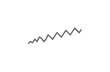
\begin{tikzpicture}[x=0.08em, y=0.08em, line width=0.4pt]
                \draw[FooterGray] (0,3) -- (1,4) -- (2,3.5) -- (3,5) -- (4,4) -- (5,6) -- (6,5.5) -- (7,4) -- (8,5) -- (9,7) -- (10,6) -- (11,5) -- (12,6.5) -- (13,8) -- (14,7) -- (15,6) -- (16,7.5) -- (17,9) -- (18,8) -- (19,7) -- (20,8.5) -- (21,10) -- (22,9) -- (23,8) -- (24,9.5);
            \end{tikzpicture}%
        }%
        \hskip0.5cm%
    }%
    \vskip6pt%
}

%=============================================================================
% PACHETE
%=============================================================================
\usepackage[utf8]{inputenc}
\usepackage[T1]{fontenc}
\usepackage{amsmath, amssymb, amsthm}
\usepackage{mathtools}
\usepackage{bm}
\usepackage{tikz}
\usetikzlibrary{arrows.meta, positioning, shapes, calc, decorations.pathreplacing, shadings}
\usepackage{booktabs}
\usepackage{multirow}
\usepackage{array}
\usepackage{graphicx}
\usepackage{hyperref}
\usepackage{colortbl}
\hypersetup{colorlinks=true, linkcolor=MainBlue, urlcolor=MainBlue}
\graphicspath{{../../logos/}{../../charts/}}
\hfuzz=2pt
\vfuzz=2pt  % Suppress tiny vertical overfull warnings (<2pt)

%=============================================================================
% COMANDA QUANTLET
%=============================================================================
\newcommand{\quantlet}[2]{%
    \hfill\href{#2}{%
        \raisebox{-0.15em}{\includegraphics[height=0.7em]{ql_logo.png}}%
        \textcolor{MainBlue}{\tiny\ #1}%
    }%
}

%=============================================================================
% PAGINĂ TITLU PERSONALIZATĂ
%=============================================================================
\defbeamertemplate*{title page}{hybrid}[1][]
{
    \vspace{0.2cm}
    % Logos row - top header (with clickable links)
    \begin{center}
        \href{https://www.ase.ro}{\includegraphics[height=1.0cm]{ase_logo.png}}\hspace{0.3cm}%
        \href{https://theida.net}{\includegraphics[height=1.0cm]{ida_logo.png}}\hspace{0.3cm}%
        \href{https://blockchain-research-center.com}{\includegraphics[height=1.0cm]{brc_logo.png}}\hspace{0.3cm}%
        \href{https://www.ai4efin.ase.ro}{\includegraphics[height=1.0cm]{ai4efin_logo.png}}\hspace{0.3cm}%
        \href{https://ipe.ro/new}{\includegraphics[height=1.0cm]{acad_logo.png}}\hspace{0.3cm}%
        \href{https://www.digital-finance-msca.com}{\includegraphics[height=1.0cm]{msca_logo.png}}%
    \end{center}

    \vspace{0.6cm}

    % Main title with Q logos on sides (with clickable links)
    \begin{center}
        \begin{minipage}{0.1\textwidth}
            \centering
            \href{https://quantlet.com}{\includegraphics[height=1.1cm]{ql_logo.png}}
        \end{minipage}%
        \begin{minipage}{0.78\textwidth}
            \centering
            {\LARGE\bfseries\usebeamercolor[fg]{title}\inserttitle}

            \vspace{0.3cm}

            {\usebeamerfont{subtitle}\usebeamercolor[fg]{title}\insertsubtitle}
        \end{minipage}%
        \begin{minipage}{0.1\textwidth}
            \centering
            \href{https://quantinar.com}{\includegraphics[height=1.1cm]{qr_logo.png}}
        \end{minipage}
    \end{center}

    \vspace{0.6cm}

    % Authors (left aligned)
    \hspace{0.5cm}{\usebeamerfont{author}\insertauthor}

    \vspace{0.3cm}

    % Institute/Affiliations (left aligned)
    \hspace{0.5cm}\begin{minipage}[t]{0.9\textwidth}
        \raggedright\small\insertinstitute
    \end{minipage}
}

%=============================================================================
% MEDII PENTRU TEOREME
%=============================================================================
\theoremstyle{definition}
\setbeamertemplate{theorems}[numbered]
\newtheorem{defn}{Definiție}
\newtheorem{thm}{Teoremă}
\newtheorem{prop}{Propoziție}
\newtheorem{rmk}{Observație}

%=============================================================================
% COMENZI PERSONALIZATE
%=============================================================================
\newcommand{\E}{\mathbb{E}}
\newcommand{\Var}{\text{Var}}
\newcommand{\Cov}{\text{Cov}}
\newcommand{\Corr}{\text{Corr}}
\newcommand{\R}{\mathbb{R}}
\newcommand{\N}{\mathbb{N}}
\newcommand{\Z}{\mathbb{Z}}
\newcommand{\RMSE}{\text{RMSE}}
\newcommand{\MAE}{\text{MAE}}
\newcommand{\MAPE}{\text{MAPE}}

%=============================================================================
% INFORMAȚII TITLU
%=============================================================================
\title[Analiza Seriilor de Timp]{Analiza și Prognoza Seriilor de Timp}
\subtitle{Capitolul 1: Procese Stochastice și Staționaritate}
\author[D.T. Pele]{Daniel Traian PELE}
\institute{Academia de Studii Economice din București\\
IDA Institute Digital Assets\\
Blockchain Research Center\\
AI4EFin Artificial Intelligence for Energy Finance\\
Academia Română, Institutul de Prognoză Economică\\
MSCA Digital Finance}
\date{}

\begin{document}

% Pagină titlu (fără antet/subsol)
{
\setbeamertemplate{headline}{}
\setbeamertemplate{footline}{}
\begin{frame}
    \titlepage
\end{frame}
}

%=============================================================================
% OBIECTIVELE CURSULUI
%=============================================================================
\begin{frame}{Obiective de Învățare}
    \begin{block}{La finalul acestui capitol, veți fi capabili să:}
    \begin{enumerate}\setlength{\itemsep}{0pt}
        \item[\textcolor{MainBlue}{\textbf{1.}}] \textbf{Definiți} procesele stochastice și să înțelegeți proprietățile acestora
        \item[\textcolor{MainBlue}{\textbf{2.}}] \textbf{Distingeți} între staționaritatea strictă și slabă (covarianță)
        \item[\textcolor{MainBlue}{\textbf{3.}}] \textbf{Identificați} procesele de zgomot alb și mers aleatoriu
        \item[\textcolor{MainBlue}{\textbf{4.}}] \textbf{Calculați} și interpretați ACF și PACF
        \item[\textcolor{MainBlue}{\textbf{5.}}] \textbf{Aplicați} operatorul lag și diferențierea
        \item[\textcolor{MainBlue}{\textbf{6.}}] \textbf{Efectuați} teste de staționaritate (ADF, KPSS)
        \item[\textcolor{MainBlue}{\textbf{7.}}] \textbf{Analizați} date financiare de tip serie de timp
        \item[\textcolor{MainBlue}{\textbf{8.}}] \textbf{Distingeți} între procesele cu rădăcină unitate și cele staționare în trend
    \end{enumerate}
    \end{block}
\end{frame}

%=============================================================================
% CUPRINS
%=============================================================================
\begin{frame}{Structura capitolului}
    \setbeamertemplate{section in toc}{\color{MainBlue}$\boxdot$~\inserttocsection}
    \tableofcontents
\end{frame}

%=============================================================================
% SECȚIUNE: MOTIVAȚIE
%=============================================================================
\section{Motivație}

\begin{frame}{Exemple: serii staționare vs. nestaționare}
    \vspace{-0.2cm}
    \begin{center}
        \includegraphics[width=\textwidth, height=0.55\textheight, keepaspectratio]{ch1_stationary_nonstationary_examples.pdf}
    \end{center}
    \vspace{-3mm}
    {\footnotesize
    \begin{exampleblock}{Observații}
    \begin{itemize}\setlength{\itemsep}{0pt}
        \item \textbf{Prețurile} (stânga) sunt nestaționare: trend, media se schimbă în timp
        \item \textbf{Randamentele} (dreapta) sunt staționare: medie $\approx 0$, varianță aprox. constantă
        \item Randamente log: $r_t = \ln P_t - \ln P_{t-1}$ $\succ$ nestaționar $\to$ staționar
    \end{itemize}
    \end{exampleblock}
    }
    \hfill\quantlet{TSA\_ch1\_stationarity}{https://github.com/QuantLet/TSA/tree/main/TSA_ch1/TSA_ch1_stationarity}
\end{frame}


%=============================================================================
% SECȚIUNEA 1: PROCESE STOCHASTICE
%=============================================================================
\section{Procese Stochastice}

\begin{frame}{Proces stochastic: definiție}
    \begin{defn}[Proces Stochastic]
        \begin{itemize}\setlength{\itemsep}{0pt}
            \item Un \textbf{proces stochastic} este o colecție de variabile aleatoare indexate după timp
            \begin{itemize}
                \item $\{X_t(\omega) : t \in \mathcal{T}, \omega \in \Omega\}$
                \item $\Omega$ este spațiul eșantion al rezultatelor posibile
            \end{itemize}
        \end{itemize}
    \end{defn}

    \vspace{0.1cm}

    \begin{columns}[T]
        \column{0.48\textwidth}
        \begin{block}{Două Perspective}
            \begin{itemize}\setlength{\itemsep}{0pt}
                \item \textbf{$\omega$ fixat}: O \textit{realizare} $\{X_t(\omega)\}_{t \in \mathcal{T}}$
                \item \textbf{$t$ fixat}: O \textit{variabilă aleatoare} $X_t$
            \end{itemize}
        \end{block}
        \column{0.5\textwidth}
        \begin{exampleblock}{Observație Cheie}
            \begin{itemize}\setlength{\itemsep}{0pt}
                \item O serie de timp pe care o observăm este \textbf{o singură realizare} a procesului stochastic subiacent
            \end{itemize}
        \end{exampleblock}
    \end{columns}
\end{frame}

\begin{frame}{Proces stochastic: ilustrare vizuală}
    \vspace{-0.2cm}
    \begin{center}
        \includegraphics[width=0.98\textwidth, height=0.60\textheight, keepaspectratio]{ch1_def_stochastic.pdf}
    \end{center}
    \vspace{-2mm}
    {\footnotesize
    \begin{exampleblock}{Interpretare}
    \begin{itemize}\setlength{\itemsep}{0pt}
        \item Fiecare linie este o \textbf{realizare diferită} din același proces stochastic subiacent
        \item Observăm doar \textbf{o singură realizare}, dar vrem să înțelegem proprietățile procesului
    \end{itemize}
    \end{exampleblock}
    }
    \hfill\quantlet{TSA\_ch1\_stationarity}{https://github.com/QuantLet/TSA/tree/main/TSA_ch1/TSA_ch1_stationarity}
\end{frame}

\begin{frame}{Momentele unui proces stochastic}
    \begin{block}{Primele Două Momente Caracterizează Procesul}
        \begin{itemize}\setlength{\itemsep}{0pt}
            \item \textbf{Funcția de Medie}: $\mu_t = \E[X_t]$
            \item \textbf{Autocovarianța (ACVF)}: $\gamma(t, s) = \Cov(X_t, X_s)$
            \begin{itemize}
                \item $\gamma(t, s) = \E[(X_t - \mu_t)(X_s - \mu_s)]$
            \end{itemize}
            \item \textbf{Autocorelația (ACF)}:
            \begin{itemize}
                \item $\rho(t, s) = \gamma(t, s) / \sqrt{\Var(X_t) \cdot \Var(X_s)}$
            \end{itemize}
        \end{itemize}
    \end{block}

    \begin{columns}[T]
        \column{0.5\textwidth}
        \begin{exampleblock}{Proprietăți ACF}
            \begin{itemize}\setlength{\itemsep}{0pt}
                \item \textbf{Interval}: $\rho(t, s) \in [-1, 1]$
                \item \textbf{Normalizare}: $\rho(t, t) = 1$ (corelație perfectă cu sine)
            \end{itemize}
        \end{exampleblock}
        \column{0.48\textwidth}
        \begin{alertblock}{Punct Cheie}
            \begin{itemize}\setlength{\itemsep}{0pt}
                \item \textbf{General}: $\mu_t$ și $\gamma(t,s)$ pot depinde de $t$
                \item \textbf{Staționar}: Elimină această dependență
            \end{itemize}
        \end{alertblock}
    \end{columns}
\end{frame}

%=============================================================================
% SECȚIUNEA 4: STAȚIONARITATE
%=============================================================================
\section{Staționaritate}

\begin{frame}{De ce contează staționaritatea}
    \vspace{-0.2cm}
    \begin{columns}[T]
        \begin{column}{0.48\textwidth}
            \begin{alertblock}{Fără Staționaritate}
            \begin{itemize}\setlength{\itemsep}{0pt}
                \item Media, varianța se schimbă în timp
                \begin{itemize}
                    \item Estimările sunt inconsistente
                \end{itemize}
                \item Trecutul poate să nu prezică viitorul
                \item Metodele standard eșuează
                \item Corelații false (spurious)
            \end{itemize}
            \end{alertblock}
        \end{column}
        \begin{column}{0.48\textwidth}
            \begin{exampleblock}{Cu Staționaritate}
            \begin{itemize}\setlength{\itemsep}{0pt}
                \item Proprietăți statistice constante
                \begin{itemize}
                    \item Ergodicitate justificată
                \end{itemize}
                \item Putem estima dintr-o singură realizare
                \item Inferență validă posibilă
                \item Modelele sunt semnificative
            \end{itemize}
            \end{exampleblock}
        \end{column}
    \end{columns}

    \begin{alertblock}{Principiu Cheie}
        \begin{itemize}\setlength{\itemsep}{0pt}
            \item Majoritatea modelelor de serii de timp (ARMA, ARIMA, etc.) necesită staționaritate
            \item Seriile nestaționare trebuie transformate (de ex., diferențiere) înainte de modelare
        \end{itemize}
    \end{alertblock}
\end{frame}

\begin{frame}{Staționaritatea strictă}
    \begin{defn}[Staționaritate Strictă (Puternică)]
        \begin{itemize}\setlength{\itemsep}{0pt}
            \item Un proces $\{X_t\}$ este \textbf{strict staționar} dacă pentru orice $k$, orice $t_1, \ldots, t_k$, și orice $h$:
            \begin{itemize}
                \item $(X_{t_1}, \ldots, X_{t_k}) \stackrel{d}{=} (X_{t_1+h}, \ldots, X_{t_k+h})$
            \end{itemize}
            \item \textbf{Notație}: $X \stackrel{d}{=} Y$ înseamnă \textit{egalitate în distribuție}
            \begin{itemize}
                \item $P(X \leq x) = P(Y \leq x)$
            \end{itemize}
        \end{itemize}
    \end{defn}

    \begin{columns}[T]
        \column{0.55\textwidth}
        \begin{block}{Implicații}
            \begin{itemize}\setlength{\itemsep}{0pt}
                \item \textbf{Distribuții identice}: $F_{X_t}(x)$ nu depinde de $t$
                \begin{itemize}
                    \item $\E[X_t] = \mu$ (medie constantă, dacă există)
                    \item $\Var(X_t) = \sigma^2$ (varianță constantă, dacă există)
                \end{itemize}
                \item \textbf{Dependența de lag}: Distribuțiile comune depind doar de lag
            \end{itemize}
        \end{block}
        \column{0.43\textwidth}
        \begin{alertblock}{Notă}
            \begin{itemize}\setlength{\itemsep}{0pt}
                \item Staționaritatea strictă este o condiție puternică, adesea imposibil de verificat în practică
            \end{itemize}
        \end{alertblock}
    \end{columns}
\end{frame}

\begin{frame}{Staționaritatea strictă: ilustrare vizuală}
    \vspace{-0.2cm}
    \begin{center}
        \includegraphics[width=0.95\textwidth, height=0.52\textheight, keepaspectratio]{ch1_def_strict_stationarity.pdf}
    \end{center}
    \vspace{-2mm}
    {\footnotesize
    \begin{exampleblock}{Interpretare}
    \begin{itemize}\setlength{\itemsep}{0pt}
        \item Translația în timp nu schimbă distribuția comună a variabilelor
        \item Oricare două ferestre temporale au aceleași proprietăți statistice
        \item În practică: verificăm doar primele momente (staționaritate slabă)
    \end{itemize}
    \end{exampleblock}
    }
    \hfill\quantlet{TSA\_ch1\_stationarity}{https://github.com/QuantLet/TSA/tree/main/TSA_ch1/TSA_ch1_stationarity}
\end{frame}

\begin{frame}{Staționaritatea slabă (covarianță)}
    \begin{defn}[Staționaritate Slabă]
        \begin{itemize}\setlength{\itemsep}{0pt}
            \item Un proces $\{X_t\}$ este \textbf{slab staționar} (sau staționar în covarianță) dacă:
            \begin{itemize}\setlength{\itemsep}{0pt}
                \item $\E[X_t^2] < \infty$ pentru toți $t$
                \begin{itemize}
                    \item Momente finite de ordin 2
                \end{itemize}
                \item $\E[X_t] = \mu$ pentru toți $t$
                \begin{itemize}
                    \item Medie constantă
                \end{itemize}
                \item $\Cov(X_t, X_{t+h}) = \gamma(h)$
                \begin{itemize}
                    \item Covarianța depinde doar de lag-ul $h$, nu de $t$
                \end{itemize}
            \end{itemize}
        \end{itemize}
    \end{defn}
    \vspace{-2mm}
    \begin{block}{Proprietăți Cheie}
    \begin{itemize}\setlength{\itemsep}{0pt}
        \item \textbf{Autocovarianța} este funcție doar de lag:
        \begin{itemize}
            \item $\gamma(h) = \Cov(X_t, X_{t+h}) = \E[(X_t - \mu)(X_{t+h} - \mu)]$
        \end{itemize}
        \item \textbf{Autocorelația}:
        \begin{itemize}
            \item $\rho(h) = \gamma(h)/\gamma(0) = \Cov(X_t, X_{t+h})/\Var(X_t)$
        \end{itemize}
        \item \textbf{Notă}: $\rho(0) = 1$, $|\rho(h)| \leq 1$, $\rho(h) = \rho(-h)$ (simetrie)
    \end{itemize}
    \end{block}
\end{frame}

\begin{frame}{Staționaritatea slabă: ilustrare vizuală}
    \vspace{-0.2cm}
    \begin{center}
        \includegraphics[width=0.95\textwidth, height=0.52\textheight, keepaspectratio]{ch1_def_weak_stationarity.pdf}
    \end{center}
    \vspace{-2mm}
    {\footnotesize
    \begin{exampleblock}{Cele trei condiții}
    \begin{itemize}\setlength{\itemsep}{0pt}
        \item $\E[X_t] = \mu$ constantă $\succ$ media nu depinde de timp
        \item $\Var(X_t) = \sigma^2$ constantă $\succ$ varianța nu depinde de timp
        \item $\Cov(X_t, X_{t+h}) = \gamma(h)$ $\succ$ autocovarianța depinde doar de lag $h$
    \end{itemize}
    \end{exampleblock}
    }
    \hfill\quantlet{TSA\_ch1\_stationarity}{https://github.com/QuantLet/TSA/tree/main/TSA_ch1/TSA_ch1_stationarity}
\end{frame}

\begin{frame}{Relația între staționaritate strictă și slabă}
    \begin{thm}[Implicație Fundamentală]
        Dacă $\{X_t\}$ este \textbf{strict staționar} și $\E[X_t^2] < \infty$, atunci $\{X_t\}$ este și \textbf{slab staționar}.
    \end{thm}

    \begin{proof}[Demonstrație]
        \begin{itemize}\setlength{\itemsep}{0pt}
            \item Fie $t_1, t_2$ oarecare și $h$ deplasare temporală arbitrară
            \item Din invarianța distribuției comune: $(X_{t_1}, X_{t_2}) \stackrel{d}{=} (X_{t_1+h}, X_{t_2+h})$
            \item $\E[X_{t_1}] = \E[X_{t_1+h}] = \mu$ (medie constantă)
            \item $\Cov(X_{t_1}, X_{t_2}) = \Cov(X_{t_1+h}, X_{t_2+h})$
            \item Deci autocovarianța depinde doar de diferența $t_2 - t_1 = h$, nu de $t_1$
        \end{itemize}
    \end{proof}

    \begin{alertblock}{Atenție: Reciproca NU este adevărată!}
        \begin{itemize}\setlength{\itemsep}{0pt}
            \item Există procese slab staționare dar \textbf{nu} strict staționare
        \end{itemize}
    \end{alertblock}
\end{frame}

\begin{frame}{Contraexemplu: slab staționar dar NU strict staționar}
    \vspace{-0.3cm}
    {\footnotesize
    \begin{exampleblock}{Construcție}
        \begin{itemize}\setlength{\itemsep}{0pt}
            \item Fie $\{X_t\}$ variabile aleatoare \textbf{independente} cu:
            $t$ par: $X_t \sim N(0, 1)$; \quad $t$ impar: $X_t \sim \frac{\chi^2(5) - 5}{\sqrt{10}}$
        \end{itemize}
    \end{exampleblock}
    }
    \vspace{-3mm}
    \begin{center}
        \includegraphics[width=0.95\textwidth, height=0.40\textheight, keepaspectratio]{ch1_counterexample_stationarity.pdf}
    \end{center}
    \vspace{-3mm}
    {\footnotesize
    \begin{columns}[T]
        \column{0.48\textwidth}
        \begin{exampleblock}{Slab staționar \checkmark}
        \begin{itemize}\setlength{\itemsep}{0pt}
            \item $\E[X_t]=0$, $\Var(X_t)=1$, $\Cov(X_t,X_{t+h})=0$
        \end{itemize}
        \end{exampleblock}
        \column{0.48\textwidth}
        \begin{alertblock}{NU strict staționar \texttimes}
        \begin{itemize}\setlength{\itemsep}{0pt}
            \item Asimetria diferă ($0$ vs $>0$) $\succ$ $X_1 \stackrel{d}{\neq} X_2$
        \end{itemize}
        \end{alertblock}
    \end{columns}
    }
    \hfill\quantlet{TSA\_ch1\_stationarity}{https://github.com/QuantLet/TSA/tree/main/TSA_ch1/TSA_ch1_stationarity}
\end{frame}

\begin{frame}{Proprietățile funcției de autocovarianță}
    \small
    \begin{prop}
    Pentru un proces slab staționar, ACVF $\gamma(h)$ satisface:
    \begin{itemize}\setlength{\itemsep}{0pt}
        \item \textbf{Simetrie:} $\gamma(h) = \gamma(-h)$
        \item \textbf{Maximum la zero:} $|\gamma(h)| \leq \gamma(0) = \Var(X_t)$
        \item \textbf{Definit nenegativ:} $\sum_{i,j} a_i a_j \gamma(i - j) \geq 0$ pentru orice $a_1, \ldots, a_n$
    \end{itemize}
    \end{prop}

    \begin{alertblock}{Demonstrație (prop. 3)}
    \begin{itemize}\setlength{\itemsep}{0pt}
        \item {\footnotesize $\Var\left(\sum_{i=1}^n a_i X_{t+i}\right) = \sum_{i,j} a_i a_j \gamma(i-j) \geq 0$ \quad (varianța $\geq 0$)}
    \end{itemize}
    \end{alertblock}

    \begin{exampleblock}{Implicație}
    \begin{itemize}\setlength{\itemsep}{0pt}
        \item Nu orice funcție poate fi o funcție de autocovarianță validă
    \end{itemize}
    \end{exampleblock}
\end{frame}

\begin{frame}{Ergodicitatea: fundamentul inferenței din date}
    \small
    \begin{defn}[Ergodicitate pentru Medie]
        \begin{itemize}\setlength{\itemsep}{0pt}
            \item Un proces staționar $\{X_t\}$ este \textbf{ergodic pentru medie} dacă:
            \begin{itemize}
                \item $\bar{X}_T = \frac{1}{T}\sum_{t=1}^{T} X_t \xrightarrow{P} \E[X_t] = \mu$ când $T \to \infty$
            \end{itemize}
        \end{itemize}
    \end{defn}

    \begin{alertblock}{De ce contează ergodicitatea?}
        \begin{itemize}\setlength{\itemsep}{0pt}
            \item \textbf{Problema}: Avem doar \textbf{o singură realizare} a procesului stochastic
            \item \textbf{Soluția}: Ergodicitatea permite estimarea lui $\mu$ din $\bar{X}_T$
            \begin{itemize}
                \item Media temporală convergează la media populației
                \item Fără ergodicitate, inferența statistică nu este posibilă!
            \end{itemize}
        \end{itemize}
    \end{alertblock}

    \begin{thm}[Condiție Suficientă]
        Dacă $\sum_{h=0}^{\infty} |\gamma(h)| < \infty$ (autocovarianțe absolut sumabile), procesul este ergodic.
    \end{thm}
\end{frame}

\begin{frame}{Ergodicitatea: ilustrare vizuală}
    \vspace{-2mm}
    \begin{center}
        \includegraphics[width=\textwidth, height=0.68\textheight, keepaspectratio]{ch1_ergodicity.pdf}
    \end{center}
    \vspace{-3mm}
    {\footnotesize
    \begin{itemize}\setlength{\itemsep}{0pt}
        \item \textbf{Media temporală} (o singură realizare) și \textbf{media ansamblului} (realizări multiple) converg ambele la $\mu$
        \item Ergodicitatea garantează că putem estima $\mu$ dintr-o \textbf{singură serie temporală} suficient de lungă
    \end{itemize}
    }
    \hfill\quantlet{TSA\_ch1\_stationarity}{https://github.com/QuantLet/TSA/tree/main/TSA_ch1/TSA_ch1_stationarity}
\end{frame}

\begin{frame}{Teorema de descompunere Wold}
    \small
    \begin{thm}[Wold, 1938]
        Orice proces \textbf{staționar în covarianță} $\{X_t\}$ poate fi scris ca:
        $X_t = \sum_{j=0}^{\infty} \psi_j \varepsilon_{t-j} + \eta_t$
        \begin{itemize}
            \item $\varepsilon_t \sim WN(0, \sigma^2)$ $\succ$ zgomot alb
            \begin{itemize}
                \item $\psi_0 = 1$, $\sum \psi_j^2 < \infty$
            \end{itemize}
            \item $\eta_t$ $\succ$ componenta deterministă (perfect predictibilă)
        \end{itemize}
    \end{thm}

    \begin{exampleblock}{Semnificația Teoremei Wold}
        \begin{itemize}\setlength{\itemsep}{0pt}
            \item \textbf{Descompunere}: Orice proces staționar = \textbf{MA($\infty$)} + componentă deterministă
            \begin{itemize}
                \item Justifică teoretic modelele MA($q$) și ARMA($p,q$)
                \item Coeficienții $\psi_j$ măsoară impactul șocurilor trecute
            \end{itemize}
        \end{itemize}
    \end{exampleblock}
\end{frame}

\begin{frame}{Teorema Wold: ilustrare vizuală}
    \begin{center}
        \includegraphics[height=4.0cm]{../../charts/ch1_wold_decomposition.pdf}
    \end{center}
    \vspace{-2mm}
    {\footnotesize
    \begin{exampleblock}{Interpretare}
    \begin{itemize}\setlength{\itemsep}{0pt}
        \item $X_t$ se descompune în componentă \textbf{stochastică} (MA($\infty$)) și componentă \textbf{deterministă} ($\eta_t$)
        \item Coeficienții $\psi_j$ descresc $\succ$ șocurile recente au impact mai mare decât cele îndepărtate
    \end{itemize}
    \end{exampleblock}
    }
    \hfill\quantlet{TSA\_ch1\_operators}{https://github.com/QuantLet/TSA/tree/main/TSA_ch1/TSA_ch1_operators}
\end{frame}

%=============================================================================
% SECȚIUNEA 5: OPERATORUL LAG, DIFERENȚIEREA ȘI TRANSFORMĂRI
%=============================================================================
\section{Operatorul lag și Diferențierea}

\begin{frame}{Operatorul lag}
    \begin{defn}[Operatorul lag]
        \begin{itemize}\setlength{\itemsep}{0pt}
            \item \textbf{Operatorul lag} (sau operatorul de întârziere) $L$ este definit prin: $LX_t = X_{t-1}$
        \end{itemize}
    \end{defn}

    \begin{columns}[T]
        \column{0.48\textwidth}
        \begin{block}{Proprietăți}
            \begin{itemize}\setlength{\itemsep}{0pt}
                \item \textbf{Puteri}: $L^k X_t = X_{t-k}$ (întârzie cu $k$ perioade)
                \begin{itemize}
                    \item Notație compactă pentru modele
                \end{itemize}
                \item \textbf{Identitate}: $L^0 = I$
                \item \textbf{Polinom}: $(1 - \phi L)X_t = X_t - \phi X_{t-1}$
            \end{itemize}
        \end{block}
        \column{0.5\textwidth}
        \begin{exampleblock}{Exemple}
            \begin{itemize}\setlength{\itemsep}{0pt}
                \item \textbf{Prima diferență}: $(1-L)X_t = X_t - X_{t-1}$
                \item \textbf{A doua diferență}: $(1-L)^2 X_t = \Delta^2 X_t$
                \item \textbf{Sezonieră}: $(1-L^{12})X_t$
            \end{itemize}
        \end{exampleblock}
    \end{columns}
\end{frame}

\begin{frame}{Operatorul lag: ilustrare vizuală}
    \vspace{-0.3cm}
    \begin{center}
        \includegraphics[width=0.98\textwidth, height=0.55\textheight, keepaspectratio]{ch1_def_lag_operator.pdf}
    \end{center}
    \vspace{-3mm}
    {\footnotesize
    \begin{exampleblock}{Proprietăți}
    \begin{itemize}\setlength{\itemsep}{0pt}
        \item $LX_t = X_{t-1}$ $\succ$ operatorul lag deplasează seria cu o perioadă în trecut
        \item $L^k X_t = X_{t-k}$ $\succ$ deplasare cu $k$ perioade; $L^0 = I$ (identitate)
        \item \textbf{Operatorul diferență}: $\Delta = (1-L)$, astfel $\Delta X_t = X_t - X_{t-1}$
    \end{itemize}
    \end{exampleblock}
    }
    \hfill\quantlet{TSA\_ch1\_operators}{https://github.com/QuantLet/TSA/tree/main/TSA_ch1/TSA_ch1_operators}
\end{frame}

\begin{frame}{Diferențierea}
    \vspace{-0.3cm}
    {\small
    \begin{block}{De ce Diferențiem?}
    \begin{itemize}\setlength{\itemsep}{0pt}
        \item \textbf{Prima Diferență}: $\Delta X_t = X_t - X_{t-1} = (1 - L)X_t$
        \begin{itemize}
            \item Elimină trendul și rădăcina unitate
            \item Mers aleatoriu: $\Delta X_t = \varepsilon_t$
        \end{itemize}
    \end{itemize}
    \end{block}

    \begin{defn}[Proces Integrat de Ordin $d$]
        \begin{itemize}\setlength{\itemsep}{0pt}
            \item Un proces $\{X_t\}$ este \textbf{integrat de ordin $d$}, notat $X_t \sim I(d)$, dacă:
            \begin{itemize}\setlength{\itemsep}{0pt}
                \item $\Delta^d X_t = (1-L)^d X_t$ este staționar ($I(0)$ proces)
                \item $\Delta^{d-1} X_t$ \textbf{nu} este staționar
            \end{itemize}
        \end{itemize}
    \end{defn}

    \begin{exampleblock}{Exemple}
    \begin{itemize}\setlength{\itemsep}{0pt}
        \item $I(0)$: Proces staționar (zgomot alb, AR staționar)
        \item $I(1)$: Mers aleatoriu $\succ$ $\Delta X_t = \varepsilon_t$ este staționar
        \item $I(2)$: Necesită două diferențieri pentru staționaritate
    \end{itemize}
    \end{exampleblock}
    }
\end{frame}

\begin{frame}{Efectul diferențierii: S\&P 500}
    \vspace{-0.2cm}
    \begin{center}
        \includegraphics[width=0.98\textwidth, height=0.60\textheight, keepaspectratio]{differencing_effect.pdf}
    \end{center}
    \vspace{-2mm}
    {\footnotesize
    \begin{exampleblock}{Interpretare}
    \begin{itemize}\setlength{\itemsep}{0pt}
        \item \textbf{Sus}: Prețuri S\&P 500 $\succ$ trend clar, nestaționar ($I(1)$)
        \item \textbf{Jos}: Randamente log $r_t = \ln P_t - \ln P_{t-1}$ $\succ$ fluctuează în jurul mediei $\approx 0$, staționar
    \end{itemize}
    \end{exampleblock}
    }
    \hfill\quantlet{TSA\_ch1\_operators}{https://github.com/QuantLet/TSA/tree/main/TSA_ch1/TSA_ch1_operators}
\end{frame}

%=============================================================================
% SECȚIUNEA 6: ZGOMOT ALB ȘI MERS ALEATORIU
%=============================================================================
\section{Zgomot Alb și Mers Aleatoriu}

\begin{frame}{Procesul de zgomot alb}
    \vspace{-0.3cm}
    {\scriptsize
    \begin{defn}[Zgomot Alb]
        \begin{itemize}\setlength{\itemsep}{0pt}
            \item Un proces $\{\varepsilon_t\}$ este \textbf{zgomot alb}, notat $\varepsilon_t \sim WN(0, \sigma^2)$, dacă:
            \begin{itemize}\setlength{\itemsep}{0pt}
                \item $\E[\varepsilon_t] = 0$ pentru orice $t$ (medie zero)
                \item $\Var(\varepsilon_t) = \sigma^2$ pentru orice $t$ (varianță constantă)
                \item $\Cov(\varepsilon_t, \varepsilon_s) = 0$ pentru $t \neq s$ (necorelat)
            \end{itemize}
        \end{itemize}
    \end{defn}
    \vspace{-2mm}
    \begin{block}{ACF al Zgomotului Alb}
        \begin{itemize}\setlength{\itemsep}{0pt}
            \item Din definiție: $\gamma(0) = \sigma^2$ și $\gamma(h) = 0$ pentru $h \neq 0$;
            $\rho(h) = \begin{cases} 1 & h = 0 \\ 0 & h \neq 0 \end{cases}$
        \end{itemize}
    \end{block}
    \vspace{-2mm}
    \begin{exampleblock}{Tipuri de zgomot alb (în ordine crescătoare a restricțiilor)}
    \begin{itemize}\setlength{\itemsep}{0pt}
        \item \textbf{Slab}: necorelat, dar pot exista dependențe neliniare
        \item \textbf{Puternic}: $\varepsilon_t$ sunt \textit{independente} și identic distribuite (i.i.d.)
        \item \textbf{Gaussian}: $\varepsilon_t \stackrel{iid}{\sim} N(0, \sigma^2)$ (necorelat $\Rightarrow$ independent)
    \end{itemize}
    \end{exampleblock}
    }
\end{frame}

\begin{frame}{Zgomot alb: ilustrare vizuală}
    \begin{center}
        \includegraphics[width=\textwidth, height=0.82\textheight, keepaspectratio]{ch1_def_white_noise.pdf}
    \end{center}
    \vspace{-3mm}
    \hfill\quantlet{TSA\_ch1\_white\_noise}{https://github.com/QuantLet/TSA/tree/main/TSA_ch1/TSA_ch1_white_noise}
\end{frame}

\begin{frame}{Cele trei tipuri de zgomot alb}
    \vspace{-2mm}
    \begin{center}
        \includegraphics[width=\textwidth, height=0.48\textheight, keepaspectratio]{ch1_white_noise_types.pdf}
    \end{center}
    \vspace{-3mm}
    {\scriptsize
    \begin{exampleblock}{Relația de incluziune: \normalfont Gaussian $\subset$ Puternic (i.i.d.) $\subset$ Slab (necorelat)}
    \begin{itemize}\setlength{\itemsep}{0pt}
        \item \textbf{Slab}: $\Cov(\varepsilon_t, \varepsilon_s) = 0$, dar pot exista dependențe neliniare (ex.\ GARCH)
        \item \textbf{Puternic}: $\varepsilon_t$ sunt i.i.d.\ --- orice distribuție (ex.\ Student-$t$)
        \item \textbf{Gaussian}: $\varepsilon_t \stackrel{iid}{\sim} N(0, \sigma^2)$ --- necorelat $\Leftrightarrow$ independent
    \end{itemize}
    \end{exampleblock}
    }
    \hfill\quantlet{TSA\_ch1\_white\_noise}{https://github.com/QuantLet/TSA/tree/main/TSA_ch1/TSA_ch1_white_noise}
\end{frame}

\begin{frame}{Procesul de mers aleatoriu}
    \small
    \vspace{-3mm}
    \begin{defn}[Mers Aleatoriu]
        $X_t = X_{t-1} + \varepsilon_t$, \; $\varepsilon_t \sim WN(0, \sigma^2)$, $X_0 = 0$ \;\;
        $\Rightarrow$ \textbf{Forma explicită}: $X_t = \sum_{i=1}^{t} \varepsilon_i$
    \end{defn}
    \vspace{-2mm}
    {\footnotesize
    \begin{prop}[Proprietăți]
        \begin{itemize}\setlength{\itemsep}{0pt}
            \item $\E[X_t] = 0$
            \item $\Var(X_t) = t\sigma^2$ (crește cu timpul!)
            \item $\Cov(X_t, X_s) = \min(t, s) \cdot \sigma^2$
        \end{itemize}
    \end{prop}
    }
    \vspace{-2mm}
    {\scriptsize
    \begin{proof}[Demonstrații]
    \begin{itemize}\setlength{\itemsep}{0pt}
        \item $\E[X_t] = \E\!\bigl[\sum_{i=1}^{t} \varepsilon_i\bigr] = 0$
        \item $\Var(X_t) = \Var\!\bigl(\sum_{i=1}^{t} \varepsilon_i\bigr) = \sum_{i=1}^{t} \Var(\varepsilon_i) = t\sigma^2$ \quad (independență)
        \item $\Cov(X_t, X_s) = \min(t,s)\,\sigma^2$ \; (pentru $s \leq t$)
    \end{itemize}
    \end{proof}
    }
    \vspace{-2mm}
    \begin{alertblock}{Nestaționar!}
    {\footnotesize $\Var(X_t) = t\sigma^2$ depinde de $t$ $\succ$ mersul aleatoriu \textbf{nu este staționar}}
    \end{alertblock}
\end{frame}

\begin{frame}{Mers aleatoriu: vizualizare}
    \vspace{-0.2cm}
    \begin{center}
        \includegraphics[width=\textwidth, height=0.58\textheight, keepaspectratio]{random_walk.pdf}
    \end{center}
    \vspace{-3mm}
    {\footnotesize
    \begin{exampleblock}{Observații}
    \begin{itemize}\setlength{\itemsep}{0pt}
        \item Fiecare șoc are \textbf{efect permanent}; $\Var(X_t) = t\sigma^2$ crește liniar cu timpul
        \item \textbf{Soluție} --- diferențierea transformă în zgomot alb, $\Delta X_t = \varepsilon_t$
    \end{itemize}
    \end{exampleblock}
    }
    \hfill\quantlet{TSA\_ch1\_random\_walk}{https://github.com/QuantLet/TSA/tree/main/TSA_ch1/TSA_ch1_random_walk}
\end{frame}

\begin{frame}{Mers aleatoriu cu drift}
    \vspace{-0.3cm}
    {\footnotesize
    \begin{defn}[Mers Aleatoriu cu Drift]
        $X_t = c + X_{t-1} + \varepsilon_t$, \; $c \neq 0$ este \textbf{driftul} \;\;
        $\Rightarrow$ \textbf{Forma explicită}: $X_t = ct + \sum_{i=1}^{t} \varepsilon_i$
    \end{defn}
    \vspace{-2mm}
    \begin{prop}[Proprietăți]
        \begin{itemize}\setlength{\itemsep}{0pt}
            \item $\E[X_t] = ct$ (trend liniar)
            \item $\Var(X_t) = t\sigma^2$ (crește cu timpul)
        \end{itemize}
    \end{prop}
    \vspace{-2mm}
    \begin{alertblock}{Diferențiere}
        $\Delta X_t = c + \varepsilon_t$ \; --- constantă plus zgomot alb $\succ$ seria diferențiată este staționară
    \end{alertblock}
    \vspace{-2mm}
    \begin{exampleblock}{Importanța practică}
        \begin{itemize}\setlength{\itemsep}{0pt}
            \item PIB nominal, prețuri de acțiuni $\succ$ adesea modele ca RW cu drift
            \item Testul ADF include variante: fără constantă, cu constantă, cu constantă și trend
        \end{itemize}
    \end{exampleblock}
    }
\end{frame}

\begin{frame}{Staționaritate în trend vs.\ staționaritate în diferențe}
    \vspace{-0.2cm}
    {\footnotesize
    \begin{columns}[T]
        \column{0.48\textwidth}
        \begin{block}{Staționaritate în trend (TS)}
            \begin{itemize}\setlength{\itemsep}{1pt}
                \item \textbf{Model}: $Y_t = \alpha + \beta t + \varepsilon_t$
                \begin{itemize}
                    \item Trend \textbf{determinist}
                    \item Abaterile de la trend sunt temporare
                \end{itemize}
                \item \textbf{Soluție}: regresie pe $t$, se extrag reziduurile
                \item \textbf{Efect}: Șocurile NU au efect permanent
            \end{itemize}
        \end{block}

        \column{0.48\textwidth}
        \begin{alertblock}{Staționaritate în diferențe (DS)}
            \begin{itemize}\setlength{\itemsep}{1pt}
                \item \textbf{Model}: $Y_t = c + Y_{t-1} + \varepsilon_t$
                \begin{itemize}
                    \item Trend \textbf{stochastic}
                    \item Abaterile de la trend sunt permanente
                \end{itemize}
                \item \textbf{Soluție}: diferențiere ($\Delta Y_t$)
                \item \textbf{Efect}: Șocurile AU efect permanent
            \end{itemize}
        \end{alertblock}
    \end{columns}

    \begin{exampleblock}{De ce contează distincția?}
        \begin{itemize}\setlength{\itemsep}{0pt}
            \item \textbf{Diferențiere pe TS}: introduce rădăcină unitară artificială în MA
            \item \textbf{Regresie pe DS}: produce reziduuri \textbf{tot nestaționare}
            \item \textbf{Soluție}: Testele ADF și KPSS ajută la distincție
        \end{itemize}
    \end{exampleblock}
    }
\end{frame}

\begin{frame}{Zgomot alb vs mers aleatoriu: comparație}
    \vspace{-0.4cm}
    \begin{columns}[T]
        \column{0.32\textwidth}
        {\scriptsize
        \begin{block}{Zgomot Alb}
            \begin{itemize}\setlength{\itemsep}{0pt}
                \item Staționar
                \item $\Var = \sigma^2$ (const.)
                \item ACF $= 0$, $h \neq 0$
                \item Fără memorie
            \end{itemize}
        \end{block}
        \begin{alertblock}{Mers Aleatoriu}
            \begin{itemize}\setlength{\itemsep}{0pt}
                \item Nestaționar
                \item $\Var = t\sigma^2$ (crește)
                \item ACF $\approx 1$ (lent)
                \item Șocuri permanente
            \end{itemize}
        \end{alertblock}
        \begin{block}{Legătură}
        \begin{itemize}\setlength{\itemsep}{0pt}
            \item $\Delta X_t = \varepsilon_t$
        \end{itemize}
        \end{block}
        }
        \column{0.66\textwidth}
        \begin{center}
            \includegraphics[width=\textwidth, height=0.65\textheight, keepaspectratio]{ch1_wn_rw.pdf}
        \end{center}
        \vspace{-3mm}
        \hfill\quantlet{TSA\_ch1\_random\_walk}{https://github.com/QuantLet/TSA/tree/main/TSA_ch1/TSA_ch1_random_walk}
    \end{columns}
\end{frame}

\begin{frame}{Comparație ACF: staționar vs mers aleatoriu}
    \vspace{-0.2cm}
    \begin{center}
        \includegraphics[width=0.95\textwidth, height=0.52\textheight, keepaspectratio]{rw_vs_stationary.pdf}
    \end{center}
    \vspace{-2mm}
    {\footnotesize
    \begin{exampleblock}{Interpretare}
    \begin{itemize}\setlength{\itemsep}{0pt}
        \item \textbf{Staționar}: ACF scade rapid (exponențial sau oscilant) spre zero
        \item \textbf{Mers aleatoriu}: ACF scade foarte lent, rămâne aproape de 1
        \item \textbf{Regulă practică}: ACF lent $\succ$ suspectăm rădăcină unitate $\succ$ test ADF
    \end{itemize}
    \end{exampleblock}
    }
    \hfill\quantlet{TSA\_ch1\_random\_walk}{https://github.com/QuantLet/TSA/tree/main/TSA_ch1/TSA_ch1_random_walk}
\end{frame}

%=============================================================================
% SECȚIUNEA 6: ACF ȘI PACF
%=============================================================================
\section{Funcții de Autocorelație}

\begin{frame}{Funcția de autocorelație eșantion}
    \vspace{-0.2cm}
    {\small
    \begin{block}{ACF Eșantion la Lag-ul $h$}
        \begin{itemize}\setlength{\itemsep}{0pt}
            \item $\hat{\rho}(h) = \frac{\sum_{t=1}^{T-h}(x_t - \bar{x})(x_{t+h} - \bar{x})}{\sum_{t=1}^{T}(x_t - \bar{x})^2}$
            \begin{itemize}
                \item Proprietăți: $\hat{\rho}(0) = 1$, $|\hat{\rho}(h)| \leq 1$
            \end{itemize}
        \end{itemize}
    \end{block}

    \begin{thm}[Bartlett, 1946]
        Sub $H_0$: zgomot alb, pentru $T$ mare: $\hat{\rho}(h) \approx N(0, 1/T)$
    \end{thm}

    \begin{block}{Interval de încredere 95\%}
    \begin{itemize}\setlength{\itemsep}{0pt}
        \item $\pm 1.96/\sqrt{T}$ (benzile din graficele ACF)
    \end{itemize}
    \end{block}

    \begin{alertblock}{Atenție}
        \begin{itemize}\setlength{\itemsep}{0pt}
            \item Formula Bartlett validă \textbf{doar sub $H_0$: zgomot alb}
            \item Pentru AR/MA, varianța asimptotică diferă
        \end{itemize}
    \end{alertblock}
    }
\end{frame}

\begin{frame}{Tipare ACF pentru diferite procese}
    \vspace{-0.3cm}
    \begin{center}
        \includegraphics[width=0.99\textwidth, height=0.60\textheight, keepaspectratio]{ch1_acf_examples.pdf}
    \end{center}
    \vspace{-3mm}
    {\footnotesize
    \begin{exampleblock}{Interpretare}
    \begin{itemize}\setlength{\itemsep}{0pt}
        \item \textbf{Zgomot alb}: ACF = 0; \textbf{Staționar}: scade rapid; \textbf{Nestaționar}: scade lent
        \item \textbf{Sezonier}: Vârfuri la lag-uri sezonale (12, 24 pentru date lunare)
    \end{itemize}
    \end{exampleblock}
    }
    \hfill\quantlet{TSA\_ch1\_acf\_patterns}{https://github.com/QuantLet/TSA/tree/main/TSA_ch1/TSA_ch1_acf_patterns}
\end{frame}

\begin{frame}{Funcția de autocorelație parțială (PACF)}
    \begin{defn}[Autocorelația Parțială]
        \begin{itemize}\setlength{\itemsep}{0pt}
            \item \textbf{PACF} la lag-ul $h$, notat $\phi_{hh}$: ultimul coeficient din regresia:
            \begin{itemize}
                \item $X_t = \phi_{h1}X_{t-1} + \phi_{h2}X_{t-2} + \cdots + \phi_{hh}X_{t-h} + e_t$
            \end{itemize}
            \item \textbf{Alternativ}:
            \begin{itemize}
                \item $\phi_{hh} = \Corr(X_t - \hat{X}_t^{(h-1)}, X_{t-h} - \hat{X}_{t-h}^{(h-1)})$
            \end{itemize}
            \item \textbf{Interpretare}: Dependența \textit{directă} la lag-ul $h$
            \begin{itemize}
                \item Elimină efectul lag-urilor intermediare
            \end{itemize}
        \end{itemize}
    \end{defn}

    \begin{exampleblock}{Aplicație Cheie: Identificarea Ordinului Modelului}
        \begin{itemize}\setlength{\itemsep}{0pt}
            \item \textbf{AR($p$)}: PACF \textbf{se anulează} după lag-ul $p$
            \begin{itemize}
                \item ACF scade exponențial sau oscilant
            \end{itemize}
            \item \textbf{MA($q$)}: ACF \textbf{se anulează} după lag-ul $q$
            \begin{itemize}
                \item PACF scade exponențial sau oscilant
            \end{itemize}
        \end{itemize}
    \end{exampleblock}
\end{frame}

\begin{frame}{Tipare ACF și PACF}
    \vspace{-0.2cm}
    \begin{center}
        \includegraphics[width=0.98\textwidth, height=0.53\textheight, keepaspectratio]{acf_pacf_examples.pdf}
    \end{center}
    \vspace{-2mm}
    {\footnotesize
    \begin{exampleblock}{Reguli de identificare}
    \begin{itemize}\setlength{\itemsep}{0pt}
        \item \textbf{AR($p$)}: ACF scade exponențial, PACF se anulează după lag $p$
        \item \textbf{MA($q$)}: ACF se anulează după lag $q$, PACF scade exponențial
        \item \textbf{ARMA($p,q$)}: Ambele scad exponențial $\succ$ identificarea necesită criterii informaționale
    \end{itemize}
    \end{exampleblock}
    }
    \hfill\quantlet{TSA\_ch1\_acf\_patterns}{https://github.com/QuantLet/TSA/tree/main/TSA_ch1/TSA_ch1_acf_patterns}
\end{frame}

\begin{frame}{Tipare de scădere ACF}
    \vspace{-0.2cm}
    \begin{center}
        \includegraphics[width=0.98\textwidth, height=0.53\textheight, keepaspectratio]{acf_theoretical.pdf}
    \end{center}
    \vspace{-2mm}
    {\footnotesize
    \begin{exampleblock}{Interpretare}
    \begin{itemize}\setlength{\itemsep}{0pt}
        \item \textbf{Scădere exponențială}: Dependență pozitivă persistentă (AR cu $\phi > 0$)
        \item \textbf{Scădere oscilantă}: Dependență alternantă (AR cu $\phi < 0$)
        \item Viteza de scădere indică puterea memoriei procesului
    \end{itemize}
    \end{exampleblock}
    }
    \hfill\quantlet{TSA\_ch1\_acf\_patterns}{https://github.com/QuantLet/TSA/tree/main/TSA_ch1/TSA_ch1_acf_patterns}
\end{frame}

%=============================================================================
% SECȚIUNEA 7: TESTAREA STAȚIONARITĂȚII
%=============================================================================
\section{Testarea Staționarității}

\begin{frame}{Testul Augmented Dickey-Fuller (ADF)}
    \vspace{-0.3cm}
    {\footnotesize
    \begin{block}{Modelul ADF}
    $\Delta X_t = \alpha + \gamma X_{t-1} + \sum_{i=1}^{p} \delta_i \Delta X_{t-i} + \varepsilon_t$, \;\;
    $\gamma = \rho - 1$, \; $H_0: \gamma = 0 \Leftrightarrow \rho = 1$
    \end{block}
    \vspace{-2mm}
    \begin{columns}[T]
        \begin{column}{0.48\textwidth}
            \begin{exampleblock}{Ipoteze}
                \begin{itemize}\setlength{\itemsep}{0pt}
                    \item \textbf{$H_0$}: $\gamma = 0$ (rădăcină unitate)
                    \item \textbf{$H_1$}: $\gamma < 0$ (staționar)
                \end{itemize}
            \end{exampleblock}
        \end{column}
        \begin{column}{0.48\textwidth}
            \begin{block}{Statistica de Test}
                \begin{itemize}\setlength{\itemsep}{0pt}
                    \item $\tau_{ADF} = \hat{\gamma}\, / \, SE(\hat{\gamma})$
                    \item $\hat{\gamma}$ = coeficient OLS al $X_{t-1}$
                    \item $SE(\hat{\gamma}) = \hat{\sigma}_\varepsilon / \sqrt{\sum X_{t-1}^2}$
                \end{itemize}
            \end{block}
        \end{column}
    \end{columns}
    \vspace{-1mm}
    \begin{alertblock}{Regula de Decizie}
        \begin{itemize}\setlength{\itemsep}{0pt}
            \item $\tau_{ADF} <$ val.\ critică $\succ$ Respingem $H_0$ $\succ$ \textcolor{Forest}{Staționar}
            \item $\tau_{ADF} \geq$ val.\ critică $\succ$ \textcolor{Crimson}{Nestaționar (rădăcină unitate)}
            \item Valorile critice urmează distribuția Dickey-Fuller (\textbf{nu} $t$-Student!)
        \end{itemize}
    \end{alertblock}
    }
\end{frame}

\begin{frame}{Testul KPSS}
    \begin{block}{Modelul}
        \begin{itemize}\setlength{\itemsep}{0pt}
            \item $X_t = \xi t + r_t + \varepsilon_t$ unde $r_t = r_{t-1} + u_t$
        \end{itemize}
    \end{block}

    \vspace{0.1cm}

    \begin{columns}[T]
        \begin{column}{0.48\textwidth}
            \begin{exampleblock}{Ipoteze (opus ADF)}
                \begin{itemize}\setlength{\itemsep}{0pt}
                    \item \textbf{$H_0$}: $\sigma_u^2 = 0$ (staționar)
                    \item \textbf{$H_1$}: $\sigma_u^2 > 0$ (rădăcină unitate)
                \end{itemize}
            \end{exampleblock}
        \end{column}
        \begin{column}{0.48\textwidth}
            \begin{block}{Statistica de Test}
                \begin{itemize}\setlength{\itemsep}{0pt}
                    \item $LM = \frac{\sum_{t=1}^{T} S_t^2}{T^2 \hat{\sigma}^2}$
                    \item {\small unde $S_t = \sum_{i=1}^{t} \hat{e}_i$}
                \end{itemize}
            \end{block}
        \end{column}
    \end{columns}

    \vspace{0.1cm}

    \begin{alertblock}{Regula de Decizie}
        \begin{itemize}\setlength{\itemsep}{0pt}
            \item $LM >$ valoarea critică $\succ$ Respingem $H_0$ $\succ$ \textcolor{Crimson}{Nestaționar}
            \item $LM \leq$ valoarea critică $\succ$ \textcolor{Forest}{Staționar}
        \end{itemize}
    \end{alertblock}
\end{frame}

\begin{frame}{Folosirea ADF și KPSS împreună}
    \begin{columns}[T]
        \column{0.55\textwidth}
        \begin{block}{Testare Confirmatorie}
            \begin{itemize}\setlength{\itemsep}{0pt}
                \item \textbf{ADF respinge $H_0$ + KPSS nu respinge}: \textcolor{Forest}{Staționar}
                \item \textbf{ADF nu respinge + KPSS respinge $H_0$}: \textcolor{Crimson}{Rădăcină Unitară}
                \item \textbf{Ambele resping sau ambele nu resping}: Neconcludent
                \begin{itemize}
                    \item Necesită teste suplimentare (PP, DF-GLS)
                \end{itemize}
            \end{itemize}
        \end{block}
        \column{0.43\textwidth}
        \begin{exampleblock}{Flux de Lucru}
            \begin{itemize}\setlength{\itemsep}{0pt}
                \item \textbf{Pasul 1}: Test ADF ($H_0$: rădăcină)
                \item \textbf{Pasul 2}: Test KPSS ($H_0$: staționar)
                \item \textbf{Pasul 3}: Rezultate concordante $\succ$ OK
                \begin{itemize}
                    \item Altfel: teste PP, DF-GLS
                \end{itemize}
            \end{itemize}
        \end{exampleblock}
    \end{columns}
\end{frame}

\begin{frame}{Testul ADF: vizualizare cu S\&P 500}
    \vspace{-0.3cm}
    \begin{center}
        \includegraphics[width=0.95\textwidth, height=0.50\textheight, keepaspectratio]{adf_test_visualization.pdf}
    \end{center}
    \vspace{-2mm}
    \quantlet{TSA\_ch1\_unit\_root\_tests}{https://github.com/QuantLet/TSA/tree/main/TSA_ch1/TSA_ch1_unit_root_tests}
    \vspace{-0.2cm}
    {\footnotesize
    \begin{block}{Interpretarea Testului ADF}
        \begin{itemize}\setlength{\itemsep}{0pt}
            \item \textbf{Ipoteza}: $H_0$: Rădăcină unitate
            \begin{itemize}
                \item Valori critice: $-3.43$ (1\%), $-2.86$ (5\%), $-2.57$ (10\%)
                \item $\tau <$ val. critică $\succ$ respingem $H_0$ $\succ$ serie staționară
            \end{itemize}
            \item \textbf{S\&P 500}: Prețuri nestaționare; Randamente staționare
        \end{itemize}
    \end{block}
    }
\end{frame}

%=============================================================================
% SECȚIUNEA 9: APLICAȚIE PE DATE REALE
%=============================================================================
\section{Aplicație pe Date Financiare}

\begin{frame}{Analiza S\&P 500: prezentare generală}
    \vspace{-0.2cm}
    \begin{center}
        \includegraphics[width=0.98\textwidth, height=0.58\textheight, keepaspectratio]{sp500_analysis.pdf}
    \end{center}
    \vspace{-2mm}
    {\footnotesize
    \begin{exampleblock}{Observații}
    \begin{itemize}\setlength{\itemsep}{0pt}
        \item \textbf{Prețuri}: Trend ascendent, nestaționar; \textbf{Randamente}: Medie $\approx 0$, staționar
        \item \textbf{ACF randamente}: $\approx 0$ (eficient); \textbf{ACF $r_t^2$}: Semnificativ (volatility clustering)
    \end{itemize}
    \end{exampleblock}
    }
    \hfill\quantlet{TSA\_ch1\_ts\_basics}{https://github.com/QuantLet/TSA/tree/main/TSA_ch1/TSA_ch1_ts_basics}
\end{frame}

\begin{frame}{Fapte stilizate ale randamentelor financiare}
    \begin{center}
        \includegraphics[width=0.95\textwidth, height=0.48\textheight, keepaspectratio]{returns_distribution.pdf}
    \end{center}
    \vspace{-0.1cm}
    \begin{columns}[T]
        \begin{column}{0.48\textwidth}
            {\footnotesize
            \begin{block}{Proprietăți observate}
            \begin{itemize}\setlength{\itemsep}{0pt}
                \item Asimetrie negativă (coadă stângă)
                \item Kurtosis excesiv ($\gg 3$)
                \item Cozi groase (heavy tails)
            \end{itemize}
            \end{block}
            }
        \end{column}
        \begin{column}{0.48\textwidth}
            {\footnotesize
            \begin{alertblock}{Implicații}
            \begin{itemize}\setlength{\itemsep}{0pt}
                \item Distribuția normală inadecvată
                \item Evenimente extreme mai probabile
                \item Necesită Student-t sau GED
            \end{itemize}
            \end{alertblock}
            }
        \end{column}
    \end{columns}
    \hfill\quantlet{TSA\_ch1\_ts\_basics}{https://github.com/QuantLet/TSA/tree/main/TSA_ch1/TSA_ch1_ts_basics}
\end{frame}

\begin{frame}{Volatility clustering}
    \vspace{-0.3cm}
    \begin{center}
        \includegraphics[width=0.95\textwidth, height=0.52\textheight, keepaspectratio]{volatility_clustering.pdf}
    \end{center}
    \vspace{-2mm}
    {\footnotesize
    \begin{exampleblock}{Observații}
    \begin{itemize}\setlength{\itemsep}{0pt}
        \item Randamente mari (în valoare absolută) urmate de randamente mari
        \item Perioade de calm urmate de perioade de calm
        \item \textbf{Volatilitate variabilă în timp} $\succ$ modele ARCH/GARCH (Cap. 5)
    \end{itemize}
    \end{exampleblock}
    }
    \hfill\quantlet{TSA\_ch1\_ts\_basics}{https://github.com/QuantLet/TSA/tree/main/TSA_ch1/TSA_ch1_ts_basics}
\end{frame}

%=============================================================================
% STUDIU DE CAZ
%=============================================================================
\section{Studiu de Caz: Testarea Staționarității}

\begin{frame}{Studiu de caz: PIB-ul trimestrial al României}
    \vspace{-0.3cm}
    \begin{center}
        \includegraphics[width=0.95\textwidth, height=0.50\textheight, keepaspectratio]{ch1_case_gdp_raw.pdf}
    \end{center}
    \vspace{-2mm}
    \quantlet{TSA\_ch1\_case\_gdp}{https://github.com/QuantLet/TSA/tree/main/TSA_ch1/TSA_ch1_case_gdp}
    \vspace{-0.2cm}
    {\footnotesize
    \begin{block}{Analiza Inițială}
        \begin{itemize}\setlength{\itemsep}{0pt}
            \item \textbf{Date}: PIB trimestrial România 2010--2023 (56 obs., INS/Eurostat)
            \item \textbf{Observații}: Trend ascendent, posibil sezonier
            \begin{itemize}
                \item Șoc structural COVID-19 vizibil
            \end{itemize}
            \item \textbf{Ipoteză}: Serie nestaționară $\succ$ testăm cu ADF și KPSS
        \end{itemize}
    \end{block}
    }
\end{frame}

\begin{frame}{Testarea staționarității: ADF și KPSS}
    \begin{columns}[T]
        \column{0.48\textwidth}
        \begin{block}{Testul ADF}
            \begin{itemize}\setlength{\itemsep}{0pt}
                \item \textbf{Ipoteză}: $H_0$: Rădăcină unitate
                \item \textbf{Rezultat}: Stat. ADF: $-1.23$
                \begin{itemize}
                    \item Val. critică: $-2.89$
                    \item Nu respingem $H_0$
                \end{itemize}
            \end{itemize}
        \end{block}
        \column{0.48\textwidth}
        \begin{exampleblock}{Testul KPSS}
            \begin{itemize}\setlength{\itemsep}{0pt}
                \item \textbf{Ipoteză}: $H_0$: Staționară
                \item \textbf{Rezultat}: Stat. KPSS: $0.89$
                \begin{itemize}
                    \item Val. critică: $0.46$
                    \item Respingem $H_0$
                \end{itemize}
            \end{itemize}
        \end{exampleblock}
    \end{columns}
    \vspace{0.2cm}
    \begin{alertblock}{Concluzie: Ambele Teste Concordă}
        \begin{itemize}\setlength{\itemsep}{0pt}
            \item Seria PIB este \textbf{nestaționară} $\succ$ necesită diferențiere
        \end{itemize}
    \end{alertblock}
\end{frame}

\begin{frame}{Diferențierea: obținerea staționarității}
    \begin{columns}[T]
        \column{0.48\textwidth}
        \begin{alertblock}{După Diferențiere}
            \begin{itemize}\setlength{\itemsep}{0pt}
                \item \textbf{Teste}: Ambele confirmă staționaritate
                \begin{itemize}
                    \item ADF: $-4.56$ (p < 0.01)
                    \item KPSS: $0.21$ (p > 0.10)
                \end{itemize}
            \end{itemize}
        \end{alertblock}
        \column{0.48\textwidth}
        \begin{exampleblock}{Concluzie}
            \begin{itemize}\setlength{\itemsep}{0pt}
                \item \textbf{PIB nivel}: nestaționar
                \item \textbf{$\Delta$PIB}: staționar
                \begin{itemize}
                    \item Folosim $\Delta PIB_t$ pentru modelare
                \end{itemize}
            \end{itemize}
        \end{exampleblock}
    \end{columns}
    \vspace{0.2cm}
    \begin{block}{Rezultat Final}
        \begin{itemize}\setlength{\itemsep}{0pt}
            \item PIB-ul necesită o diferențiere pentru a deveni staționar
        \end{itemize}
    \end{block}
\end{frame}

%=============================================================================
\section{Utilizare IA}
%=============================================================================

\begin{frame}{Experiment: ChatGPT vs Fundamentele}
    \vspace{-2mm}
    \begin{block}{\footnotesize Prompt $\to$ Răspuns}
        {\footnotesize
        \textbf{Tu}: ``Am date zilnice cu cursul EUR/RON din ultimii 5 ani. Poți să-mi faci o prognoză pentru săptămâna viitoare?''\\[2pt]
        \textbf{ChatGPT}: ``ADF: $p = 0{,}67$ $\to$ nestaționară. După diferențiere: $p < 0{,}01$ $\to$ staționară.\\
        Am ajustat ARMA(2,1). Coeficientul $\phi_1 = 0{,}03$ semnificativ ($p = 0{,}02$). RMSE $= 0{,}0043$.''
        }
    \end{block}
    \vspace{-1mm}
    {\small
    \textbf{Exercițiu}:
    \begin{enumerate}\setlength{\itemsep}{2pt}
        \item Identificați cel puțin trei erori metodologice în analiza AI de mai sus.
        \item Descărcați date EUR/RON și reproduceți afirmațiile AI. Care dintre ele rezistă?
        \item Comparați acuratețea prognozei ARMA(2,1) cu un benchmark naiv folosind testul Diebold--Mariano.
        \item Explicați: dacă prețurile urmează un mers aleatoriu, poate \textit{vreun} model să bată $\hat{X}_{t+1} = X_t$?
    \end{enumerate}
    }
    \vspace{-1mm}
    \begin{alertblock}{}
        {\small \textbf{Discuție}: AI raportează RMSE mic și coeficienți semnificativi. \textit{E suficient pentru a avea încredere în prognoză?}}
    \end{alertblock}
\end{frame}

%=============================================================================
% REZUMAT
%=============================================================================
\section{Rezumat}

\begin{frame}{Concluzii principale}
    \begin{block}{Rezumat}
    \small
    \begin{itemize}\setlength{\itemsep}{0pt}
        \item \textbf{Proces stochastic}: colecție de variabile aleatoare indexate în timp
        \item \textbf{Staționaritate slabă}: medie, varianță, autocovarianță constante
        \item \textbf{Zgomot alb}: $\varepsilon_t \sim WN(0, \sigma^2)$
        \begin{itemize}
            \item Staționar, ACF $= 0$ pentru $h \neq 0$
        \end{itemize}
        \item \textbf{Mers aleatoriu}: $X_t = X_{t-1} + \varepsilon_t$
        \begin{itemize}
            \item Nestaționar, $\Var(X_t) = t\sigma^2$
        \end{itemize}
        \item \textbf{ACF/PACF}: instrumente cheie pentru identificarea structurii
        \item \textbf{Diferențierea}: transformă serii nestaționare în staționare
        \item \textbf{Teste rădăcină unitate}:
        \begin{itemize}
            \item ADF ($H_0$: rădăcină unitate) vs KPSS ($H_0$: staționar)
        \end{itemize}
    \end{itemize}
    \end{block}
\end{frame}

\begin{frame}{Formule importante}
    \begin{columns}[T]
        \column{0.48\textwidth}
        {\small
        \begin{block}{Staționaritate Slabă}
            \begin{itemize}\setlength{\itemsep}{0pt}
                \item \textbf{Momente constante}:
                \begin{itemize}
                    \item $\E[X_t] = \mu$ (medie constantă)
                    \item $\Var(X_t) = \sigma^2$ (varianță constantă)
                \end{itemize}
                \item \textbf{Autocovarianță}: $\gamma(h) = \Cov(X_t, X_{t+h})$
                \item \textbf{Autocorelație}: $\rho(h) = \gamma(h)/\gamma(0)$
            \end{itemize}
        \end{block}

        \begin{block}{Operatorul lag}
            \begin{itemize}\setlength{\itemsep}{0pt}
                \item \textbf{Lag}: $LX_t = X_{t-1}$
                \item \textbf{Diferență}: $\Delta X_t = (1-L)X_t$
            \end{itemize}
        \end{block}
        }

        \column{0.48\textwidth}
        {\small
        \begin{exampleblock}{Zgomot Alb (WN)}
            \begin{itemize}\setlength{\itemsep}{0pt}
                \item \textbf{Model}: $\varepsilon_t \sim WN(0, \sigma^2)$
                \item \textbf{ACF}: $\rho(h) = 0$ pentru $h \neq 0$
            \end{itemize}
        \end{exampleblock}

        \begin{alertblock}{Mers Aleatoriu (RW)}
            \begin{itemize}\setlength{\itemsep}{0pt}
                \item \textbf{Model}: $X_t = X_{t-1} + \varepsilon_t$
                \item \textbf{Varianță}: $\Var(X_t) = t\sigma^2$ (crește!)
            \end{itemize}
        \end{alertblock}
        }
    \end{columns}
\end{frame}

\begin{frame}{Previzualizare capitolul următor}
    \begin{columns}[T]
        \column{0.48\textwidth}
        \begin{block}{Capitolul 2: Modele ARMA}
            \begin{itemize}\setlength{\itemsep}{0pt}
                \item \textbf{AR($p$)}: Modele Autoregresive
                \item \textbf{MA($q$)}: Modele Medie Mobilă
                \item \textbf{ARMA($p,q$)}: Modele combinate
                \item \textbf{Identificare}: Cu ACF/PACF
            \end{itemize}
        \end{block}
        \column{0.48\textwidth}
        \begin{exampleblock}{Ce Vom Învăța}
            \begin{itemize}\setlength{\itemsep}{0pt}
                \item \textbf{Estimare}: Parametrii modelului
                \item \textbf{Diagnostic}: Verificarea modelului
                \item \textbf{Prognoză}: Intervale de încredere
                \item \textbf{Selecție}: AIC, BIC
            \end{itemize}
        \end{exampleblock}
    \end{columns}
\end{frame}

%=============================================================================
% SECȚIUNE: QUIZ
%=============================================================================
\section{Quiz}

\begin{frame}{Întrebarea 1}
    \begin{alertblock}{Întrebare}
        \begin{itemize}\setlength{\itemsep}{0pt}
            \item Care sunt cele trei condiții pentru staționaritatea slabă (în covarianță)?
        \end{itemize}
    \end{alertblock}

    \vspace{0.3cm}

    \begin{block}{Variante de răspuns}
    \begin{enumerate}[(A)]\setlength{\itemsep}{0pt}
        \item Media zero, varianța infinită, covarianță dependentă de timp
        \item Media constantă, varianța constantă, autocovarianța depinde doar de lag
        \item Distribuție normală, independență, varianță unitară
        \item Trend liniar, sezonalitate constantă, reziduuri albe
    \end{enumerate}
    \end{block}
\end{frame}

\begin{frame}{Întrebarea 1: Răspuns}
    \vspace{-0.2cm}
    \begin{center}
        \includegraphics[width=0.98\textwidth, height=0.58\textheight, keepaspectratio]{ch1_quiz2_stationarity.pdf}
    \end{center}
    \vspace{-3mm}
    {\small
    \begin{exampleblock}{Răspuns: (B)}
    \begin{itemize}\setlength{\itemsep}{0pt}
        \item $\E[X_t]=\mu$, $\Var(X_t)=\sigma^2$, $\gamma(t,s)=\gamma(|t-s|)$
    \end{itemize}
    \end{exampleblock}
    }
    \hfill\quantlet{TSA\_ch1\_stationarity}{https://github.com/QuantLet/TSA/tree/main/TSA_ch1/TSA_ch1_stationarity}
\end{frame}

\begin{frame}{Întrebarea 2}
    \begin{alertblock}{Întrebare}
        \begin{itemize}\setlength{\itemsep}{0pt}
            \item Care este ipoteza nulă ($H_0$) în testul ADF (Augmented Dickey-Fuller)?
        \end{itemize}
    \end{alertblock}

    \vspace{0.3cm}

    \begin{block}{Variante de răspuns}
    \begin{enumerate}[(A)]\setlength{\itemsep}{0pt}
        \item Seria este staționară
        \item Seria are rădăcină unitate (este nestaționară)
        \item Seria nu are autocorelație
        \item Seria are distribuție normală
    \end{enumerate}
    \end{block}
\end{frame}

\begin{frame}{Întrebarea 2: Răspuns}
    \vspace{-0.2cm}
    \begin{center}
        \includegraphics[width=0.98\textwidth, height=0.58\textheight, keepaspectratio]{adf_test_visualization.pdf}
    \end{center}
    \vspace{-3mm}
    {\small
    \begin{exampleblock}{Răspuns: (B)}
    \begin{itemize}\setlength{\itemsep}{0pt}
        \item $H_0$: rădăcină unitate; $\tau <$ val. critică $\succ$ staționară
    \end{itemize}
    \end{exampleblock}
    }
    \hfill\quantlet{TSA\_ch1\_unit\_root\_tests}{https://github.com/QuantLet/TSA/tree/main/TSA_ch1/TSA_ch1_unit_root_tests}
\end{frame}

\begin{frame}{Întrebarea 3}
    \begin{alertblock}{Întrebare}
        \begin{itemize}\setlength{\itemsep}{0pt}
            \item Care este ipoteza nulă ($H_0$) în testul KPSS?
        \end{itemize}
    \end{alertblock}

    \vspace{0.3cm}

    \begin{block}{Variante de răspuns}
    \begin{enumerate}[(A)]\setlength{\itemsep}{0pt}
        \item Seria are rădăcină unitate (nestaționară)
        \item Seria este staționară
        \item Seria este un mers aleatoriu
        \item Seria are trend determinist
    \end{enumerate}
    \end{block}
\end{frame}

\begin{frame}{Întrebarea 3: Răspuns}
    \vspace{-0.2cm}
    \begin{center}
        \includegraphics[width=0.98\textwidth, height=0.58\textheight, keepaspectratio]{ch1_stationarity.pdf}
    \end{center}
    \vspace{-3mm}
    {\small
    \begin{exampleblock}{Răspuns: (B)}
    \begin{itemize}\setlength{\itemsep}{0pt}
        \item KPSS: $H_0$ staționară (opus ADF). Folosiți ambele teste!
    \end{itemize}
    \end{exampleblock}
    }
    \hfill\quantlet{TSA\_ch1\_unit\_root\_tests}{https://github.com/QuantLet/TSA/tree/main/TSA_ch1/TSA_ch1_unit_root_tests}
\end{frame}

\begin{frame}{Întrebarea 4}
    \begin{alertblock}{Întrebare}
        \begin{itemize}\setlength{\itemsep}{0pt}
            \item Care este proprietatea cheie a varianței unui mers aleatoriu $X_t = X_{t-1} + \varepsilon_t$?
        \end{itemize}
    \end{alertblock}

    \vspace{0.3cm}

    \begin{block}{Variante de răspuns}
    \begin{enumerate}[(A)]\setlength{\itemsep}{0pt}
        \item Varianța este constantă: $\Var(X_t) = \sigma^2$
        \item Varianța crește liniar cu timpul: $\Var(X_t) = t\sigma^2$
        \item Varianța scade cu timpul
        \item Varianța este zero
    \end{enumerate}
    \end{block}
\end{frame}

\begin{frame}{Întrebarea 4: Răspuns}
    \vspace{-0.2cm}
    \begin{center}
        \includegraphics[width=0.98\textwidth, height=0.58\textheight, keepaspectratio]{ch1_quiz4_wn_rw.pdf}
    \end{center}
    \vspace{-3mm}
    {\small
    \begin{exampleblock}{Răspuns: (B)}
    \begin{itemize}\setlength{\itemsep}{0pt}
        \item $\Var(X_t) = t\sigma^2$ crește liniar $\succ$ nestaționar
    \end{itemize}
    \end{exampleblock}
    }
    \hfill\quantlet{TSA\_ch1\_random\_walk}{https://github.com/QuantLet/TSA/tree/main/TSA_ch1/TSA_ch1_random_walk}
\end{frame}

\begin{frame}{Întrebarea 5}
    \begin{alertblock}{Întrebare}
        \begin{itemize}\setlength{\itemsep}{0pt}
            \item Cum arată ACF-ul unui mers aleatoriu (serie nestaționară cu rădăcină unitate)?
        \end{itemize}
    \end{alertblock}

    \vspace{0.3cm}

    \begin{block}{Variante de răspuns}
    \begin{enumerate}[(A)]\setlength{\itemsep}{0pt}
        \item Toate valorile sunt zero după lag 0
        \item Scade exponențial rapid
        \item Scade foarte lent (persistență înaltă)
        \item Oscilează între pozitiv și negativ
    \end{enumerate}
    \end{block}
\end{frame}

\begin{frame}{Întrebarea 5: Răspuns}
    \vspace{-0.2cm}
    \begin{center}
        \includegraphics[width=0.98\textwidth, height=0.58\textheight, keepaspectratio]{rw_vs_stationary.pdf}
    \end{center}
    \vspace{-3mm}
    {\small
    \begin{exampleblock}{Răspuns: (C)}
    \begin{itemize}\setlength{\itemsep}{0pt}
        \item ACF $\approx$ 1 pentru multe lag-uri, scădere lentă $\succ$ test ADF
    \end{itemize}
    \end{exampleblock}
    }
    \hfill\quantlet{TSA\_ch1\_random\_walk}{https://github.com/QuantLet/TSA/tree/main/TSA_ch1/TSA_ch1_random_walk}
\end{frame}

\begin{frame}{Întrebarea 6}
    \begin{alertblock}{Întrebare}
        \begin{itemize}\setlength{\itemsep}{0pt}
            \item Cum obținem randamente staționare dintr-o serie de prețuri financiare $P_t$?
        \end{itemize}
    \end{alertblock}

    \vspace{0.3cm}

    \begin{block}{Variante de răspuns}
    \begin{enumerate}[(A)]\setlength{\itemsep}{0pt}
        \item Diferențiere simplă: $\Delta P_t = P_t - P_{t-1}$
        \item Logaritmare apoi diferențiere: $r_t = \ln P_t - \ln P_{t-1}$
        \item Doar logaritmare: $\ln P_t$
        \item Standardizare: $(P_t - \bar{P})/s_P$
    \end{enumerate}
    \end{block}
\end{frame}

\begin{frame}{Întrebarea 6: Răspuns}
    \vspace{-0.2cm}
    \begin{center}
        \includegraphics[width=0.98\textwidth, height=0.58\textheight, keepaspectratio]{differencing_effect.pdf}
    \end{center}
    \vspace{-3mm}
    {\small
    \begin{exampleblock}{Răspuns: (B)}
    \begin{itemize}\setlength{\itemsep}{0pt}
        \item Randamente log: $r_t = \ln P_t - \ln P_{t-1}$
        \item Mai întâi $\ln$ (stabilizează varianța), apoi $\Delta$ (elimină trendul) $\succ$ serie staționară
    \end{itemize}
    \end{exampleblock}
    }
    \hfill\quantlet{TSA\_ch1\_operators}{https://github.com/QuantLet/TSA/tree/main/TSA_ch1/TSA_ch1_operators}
\end{frame}

%=============================================================================
% BIBLIOGRAFIE
%=============================================================================
\begin{frame}{Bibliografie}
    \small
    \begin{columns}[T]
        \column{0.50\textwidth}
        \begin{block}{Manuale Fundamentale}
            {\scriptsize
            \begin{itemize}\setlength{\itemsep}{0pt}
                \item Hyndman \& Athanasopoulos (2021). \textit{Forecasting}, OTexts
                \item Shumway \& Stoffer (2017). \textit{Time Series Analysis}, Springer
                \item Hamilton (1994). \textit{Time Series Analysis}, Princeton
            \end{itemize}
            }
        \end{block}
        \begin{exampleblock}{Referințe Clasice}
            {\scriptsize
            \begin{itemize}\setlength{\itemsep}{0pt}
                \item Wold (1938). \textit{Analysis of Stationary Time Series}
                \item Bartlett (1946). ``Sampling Properties'', \textit{JRSS}
            \end{itemize}
            }
        \end{exampleblock}
        \column{0.48\textwidth}
        \begin{alertblock}{Resurse Online}
            {\scriptsize
            \begin{itemize}\setlength{\itemsep}{0pt}
                \item \textbf{Quantlet}: \url{https://quantlet.com} $\succ$ cod statistică
                \item \textbf{Quantinar}: \url{https://quantinar.com} $\succ$ tutoriale
                \item \textbf{GitHub TSA\_ch1}: \url{https://github.com/QuantLet/TSA/tree/main/TSA_ch1}
            \end{itemize}
            }
        \end{alertblock}
    \end{columns}
\end{frame}

%=============================================================================
% SURSE DE DATE
%=============================================================================
\begin{frame}{Surse de date și software}
    \begin{columns}[T]
        \column{0.48\textwidth}
        \begin{block}{Date Utilizate}
            \begin{itemize}\setlength{\itemsep}{0pt}
                \item \textbf{S\&P 500}: Yahoo Finance
                    \begin{itemize}
                        \item Prețuri, randamente
                    \end{itemize}
                \item \textbf{PIB România}: INS/Eurostat
                    \begin{itemize}
                        \item Date trimestriale
                    \end{itemize}
                \item \textbf{Cursuri valutare}: BNR
            \end{itemize}
        \end{block}
        \column{0.48\textwidth}
        \begin{exampleblock}{Software}
            \begin{itemize}\setlength{\itemsep}{0pt}
                \item \textbf{Python}: statsmodels, pandas, matplotlib, scipy
                \item \textbf{R}: forecast, tseries, urca
                \item \textbf{Date}: Yahoo Finance, FRED, Eurostat
            \end{itemize}
        \end{exampleblock}
    \end{columns}
\end{frame}

\begin{frame}{}
    \centering
    \vspace{1cm}

    \Huge\textcolor{MainBlue}{Vă Mulțumim!}

    \vspace{0.8cm}

    \Large Întrebări?

    \vspace{1cm}

    \normalsize
    Materialele cursului sunt disponibile la: \url{https://danpele.github.io/Time-Series-Analysis/}

    \vspace{0.3cm}

    \href{https://quantlet.com}{\raisebox{-0.15em}{\includegraphics[height=0.8em]{ql_logo.png}} Quantlet} \hspace{0.5cm}
    \href{https://quantinar.com}{\raisebox{-0.15em}{\includegraphics[height=0.8em]{qr_logo.png}} Quantinar}
\end{frame}

\end{document}
